\chapter{Solu\c tia propus\u a}

\section{Cerinte functionale pentru utilizator si nefunctionale}

\subsection{Cerinte funtionale pentru utilizator}

\begin{itemize}
	\item \textbf{RF-U1} --- \^Inregistrare cont: username, email, telefon, parol\u a; trimitere cod 6 cifre pe email; creare cont dup\u a verificare.
	\item \textbf{RF-U2} --- Autentificare cu email \c si parol\u a; primire token JWT.
	\item \textbf{RF-U3} --- Resetare parol\u a prin email sau telefon (email mascat la c\u autare dup\u a telefon).
	\item \textbf{RF-U4} --- Vizualizare list\u a evenimente viitoare; filtre: nume, jude\c t, dat\u a.
	\item \textbf{RF-U5} --- Pagin\u a detalii eveniment: descriere, imagini, loca\c tie, pre\c t, locuri.
	\item \textbf{RF-U6} --- Cump\u arare bilete nominale (1..N nume); redirect Stripe Checkout.
	\item \textbf{RF-U7} --- Confirmare plat\u a; vizualizare bilete \^in ``Biletele mele'' (viitoare/trecute).
	\item \textbf{RF-U8} --- Editare profil; schimbare parol\u a; \c stergere cont (cu confirmare parol\u a).
\end{itemize}

\subsection{Cerin\c te func\c tionale pentru administrator}

\begin{itemize}
	\item \textbf{RF-A1} --- CRUD evenimente: titlu, descriere, dat\u a, jude\c t, localitate, loca\c tie, pre\c t, locuri, durat\u a, imagini (max 8).
	\item \textbf{RF-A2} --- List\u a participan\c ti per eveniment; check-in.
	\item \textbf{RF-A3} --- Promovare/revocare rol admin (cu parol\u a autorizare); protec\c tie ultim admin.
\end{itemize}

\subsection{Cerin\c te nefunc\c tionale}

\begin{itemize}
	\item \textbf{RNF-1 Securitate} --- bcrypt, JWT, hash token-uri/coduri, CORS, rate limiting.
	\item \textbf{RNF-2 Disponibilitate} --- API stateless; DB rela\c tional\u a.
	\item \textbf{RNF-3 UX} --- Responsive; tem\u a dark; mesaje eroare clare.
	\item \textbf{RNF-4 Mentenabilitate} --- Separare frontend/backend; migr\u ari SQL.
	\item \textbf{RNF-5 Portabilitate} --- Node.js 18+, PostgreSQL 14+.
\end{itemize}

\section{Arhitectura sistemului}

ManFast urmeaz\u a arhitectura \textbf{client-server} \^in trei straturi:

\begin{enumerate}
	\item \textbf{Strat prezentare} --- SPA React (Vite), routing React Router, context autentificare, apeluri \texttt{fetch} c\u atre API.
	\item \textbf{Strat aplica\c tie} --- Express: rute \texttt{/api/auth}, \texttt{/api/events}, \texttt{/api/tickets}; middleware JWT \c si \texttt{requireAdmin}.
	\item \textbf{Strat date} --- PostgreSQL; fi\c siere statice imagini \^in \texttt{uploads/}.
\end{enumerate}

Servicii externe: \textbf{Stripe} (pl\u a\c ti), \textbf{Brevo SMTP} (email verificare \c si reset).


\begin{figure}[htbp]
	\centering
		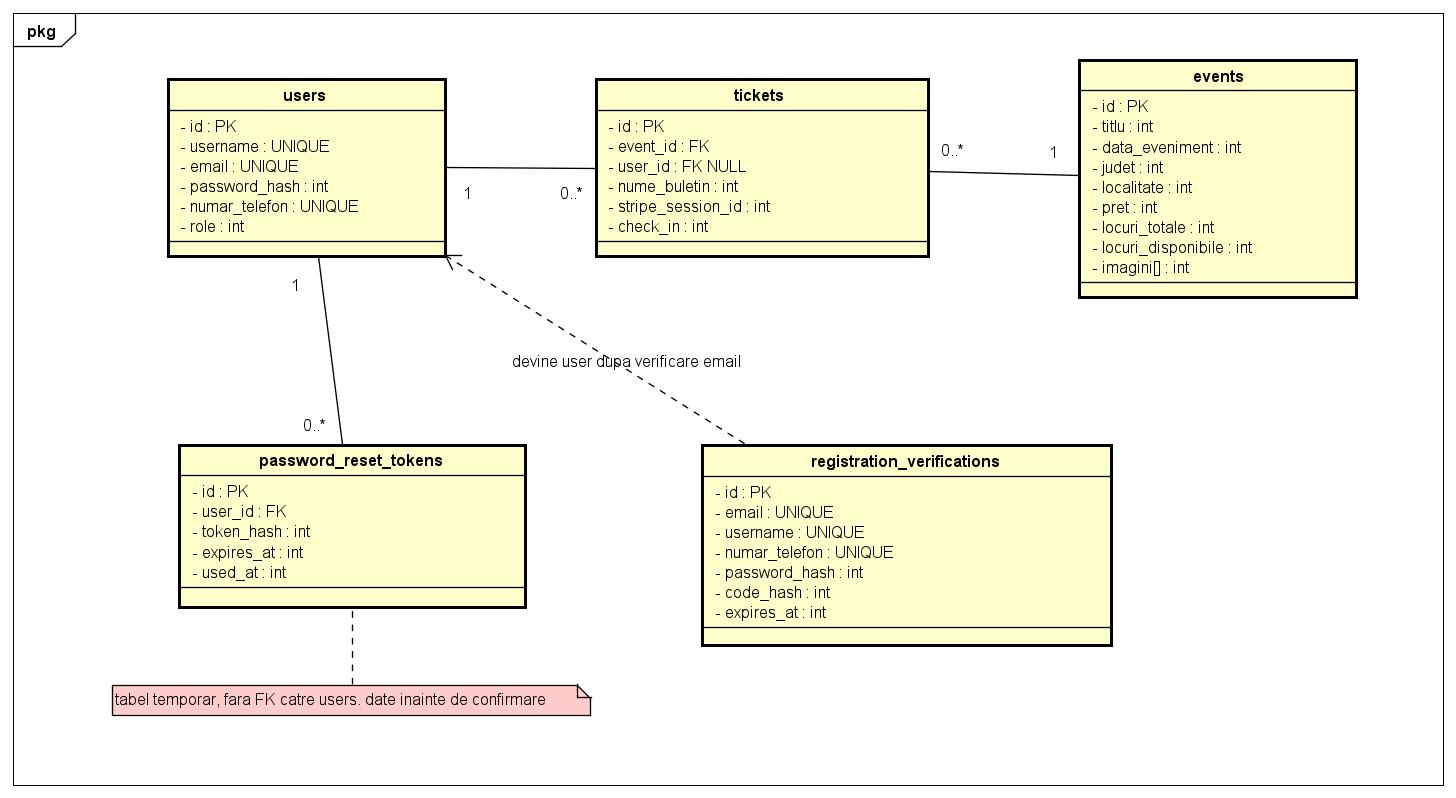
\includegraphics[width=1\textwidth]{Model de domeniu _ ERD ManFast.jpg}
	\caption{Arhitectura sistemului ManFast}
	\label{fig:l2f1}
\end{figure}

Instructiuni inserare: Diagrama blocuri: Browser (React+MUI) -> HTTPS/JSON → Express API -> PostgreSQL; lateral Stripe si Brevo SMTP. Tool: draw.io, Lucidchart sau PowerPoint. Export PNG 300dpi, latime ˜14cm ˘ in document.


\section{Tehnologii utilizate}

\begin{table}[htbp]
	\centering
	\begin{tabular}{|l|p{8cm}|}
		\hline
		\textbf{Tehnologie} & \textbf{Rol} \\
		\hline
		React 19 + Vite 8 & Frontend SPA, HMR dev \\
		\hline
		Material UI 9 & Componente UI, temă dark \\
		\hline
		Express 4 & API REST, Multer upload \\
		\hline
		PostgreSQL & Persistență relațională \\
		\hline
		JWT + bcrypt & Auth și hash parole \\
		\hline
		Stripe Checkout & Plăți card RON \\
		\hline
		Nodemailer + Brevo & Email SMTP \\
		\hline
	\end{tabular}
	\caption{Stack tehnologic ManFast}
	\label{tab:tech}
\end{table}

React [8] gestioneaza starea UI si re-renderarea eficienta.Vite ofera build rapid. Express [11] routeaza cererile HTTP. pg conecteaza la PostgreSQL. Stripe SDK creeaza sesiuni Checkout.

\section{Diagrame UML}
\subsection{Cazuri de utilizare}

Actorii principali sunt Utilizatorul (autentificat sau nu) si Administratorul. Utilizatorul
poate ınregistra cont, autentifica, filtra evenimente, cumpara bilete, gestiona profilul. Administratorul publica evenimente, face check-in, gestioneaza alti admini. 

\begin{figure}[htbp]
	\centering
	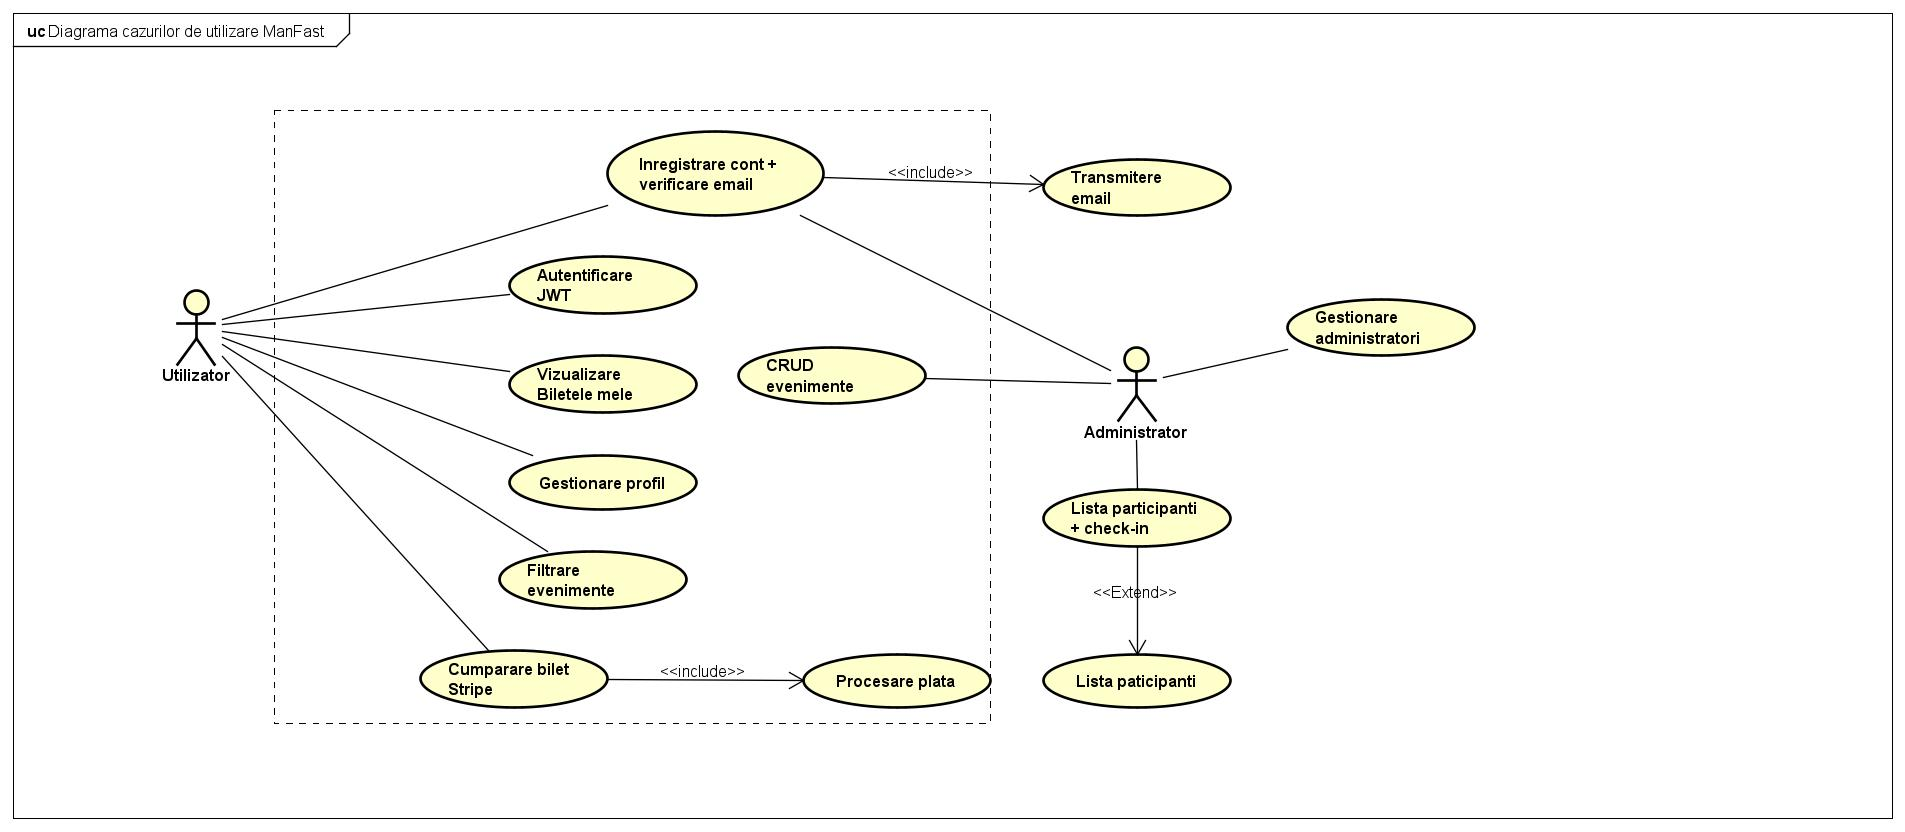
\includegraphics[width=1\textwidth]{Diagrama cazurilor de utilizare ManFast.jpg}
	\caption{ Diagrama cazurilor de utilizare}
	\label{fig:l2f1}
\end{figure}

Instructiuni inserare: UML use case: actor Utilizator (register, login, filtre, cumpara bilet, profil); actor Admin (CRUD eveniment, check-in, promovare admin). Tool: StarUML, draw.io. Include sistem boundary “ManFast”.

\subsection{Secventa de inregistrare cu verificare prin email}

Flux: Frontend POST /register-> Backend valideaza, salveaza ın {\tt registration verifications},
trimite cod SMTP -> Frontend POST /register/verify → INSERT {\tt users}.

\begin{figure}[htbp]
	\centering
	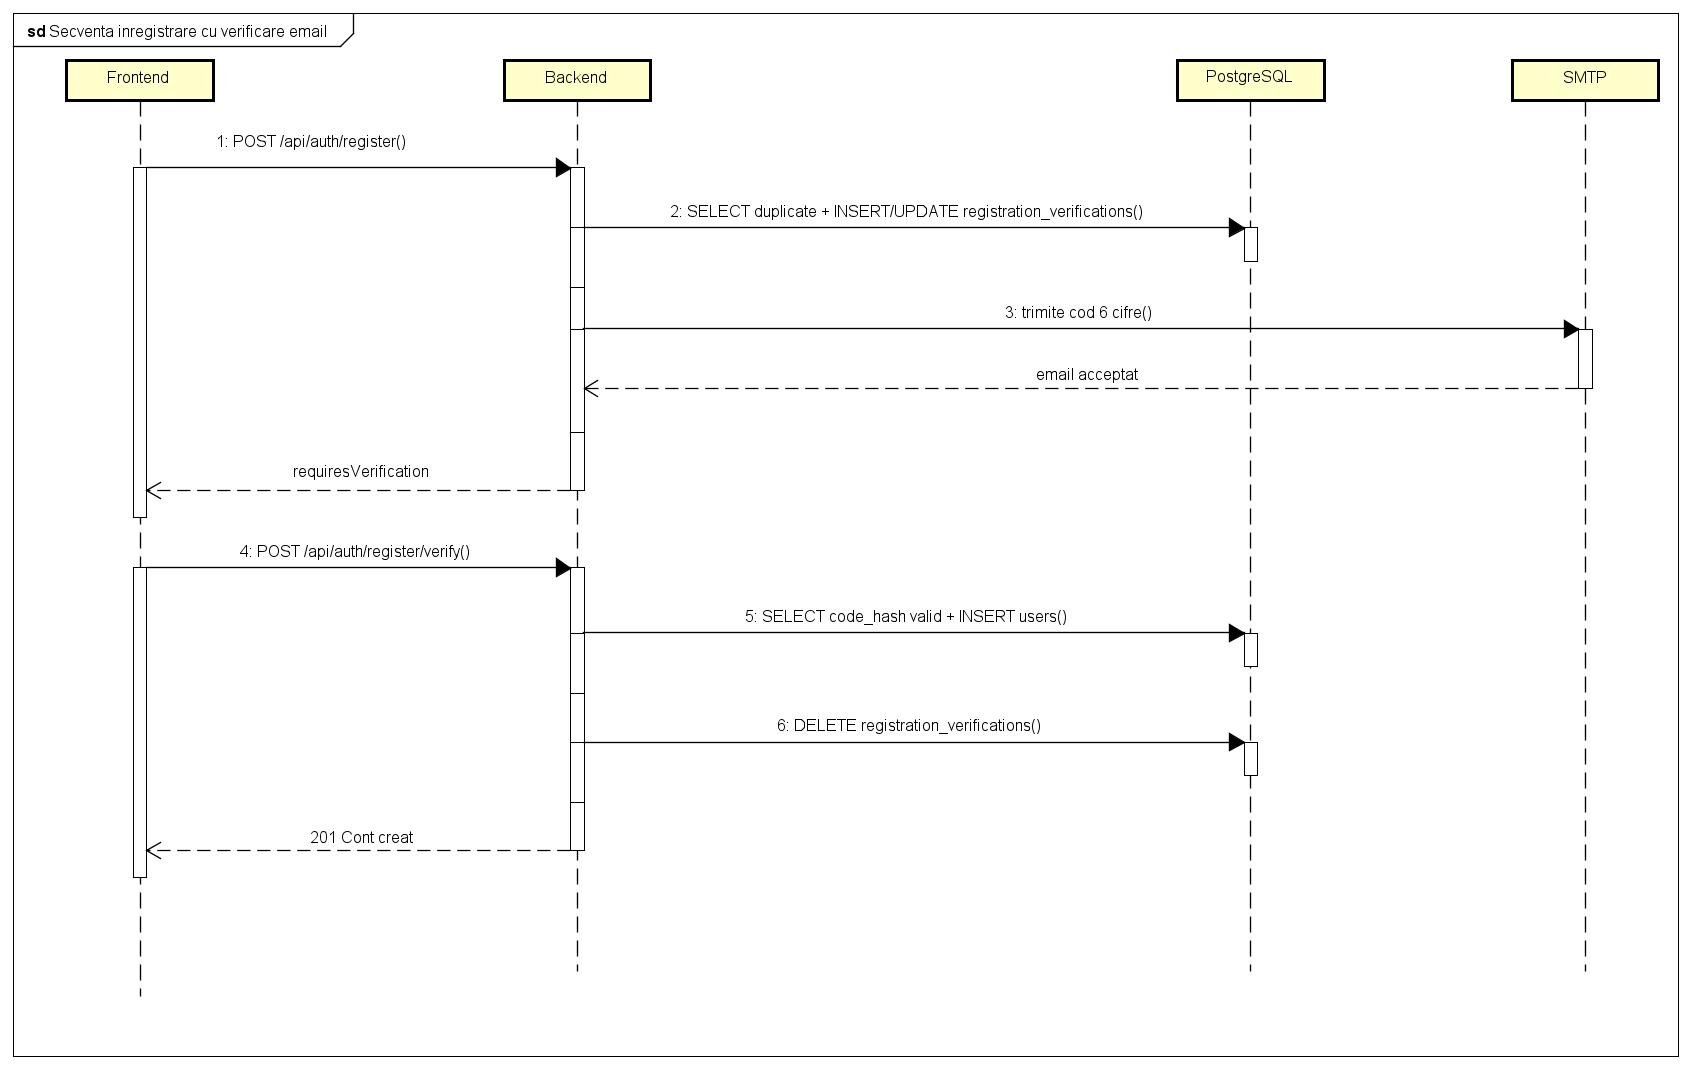
\includegraphics[width=1\textwidth]{Secventa inregistrare cu verificare email.jpg}
	\caption{Diagrama de secventa - inregistrarea cu email}
	\label{fig:l2f1}
\end{figure}

Instructiuni inserare: Participant¸i: Utilizator, Frontend, Backend, PostgreSQL, SMTP. Mesaje:
register, salveaza temp, trimite cod, verify, creare user. Notat¸ii pe fiecare sageata.

\subsection{Secventa pentru plata prin Stripe}

Flux: Frontend POST create-checkout-session → redirect Stripe → success URL → confirmpayment → INSERT tickets, UPDATE locuri.

Instructiuni inserare: Participant¸i: Utilizator, Frontend, Backend, Stripe, DB. Include metadata session si confirm-payment.

\begin{figure}[htbp]
	\centering
	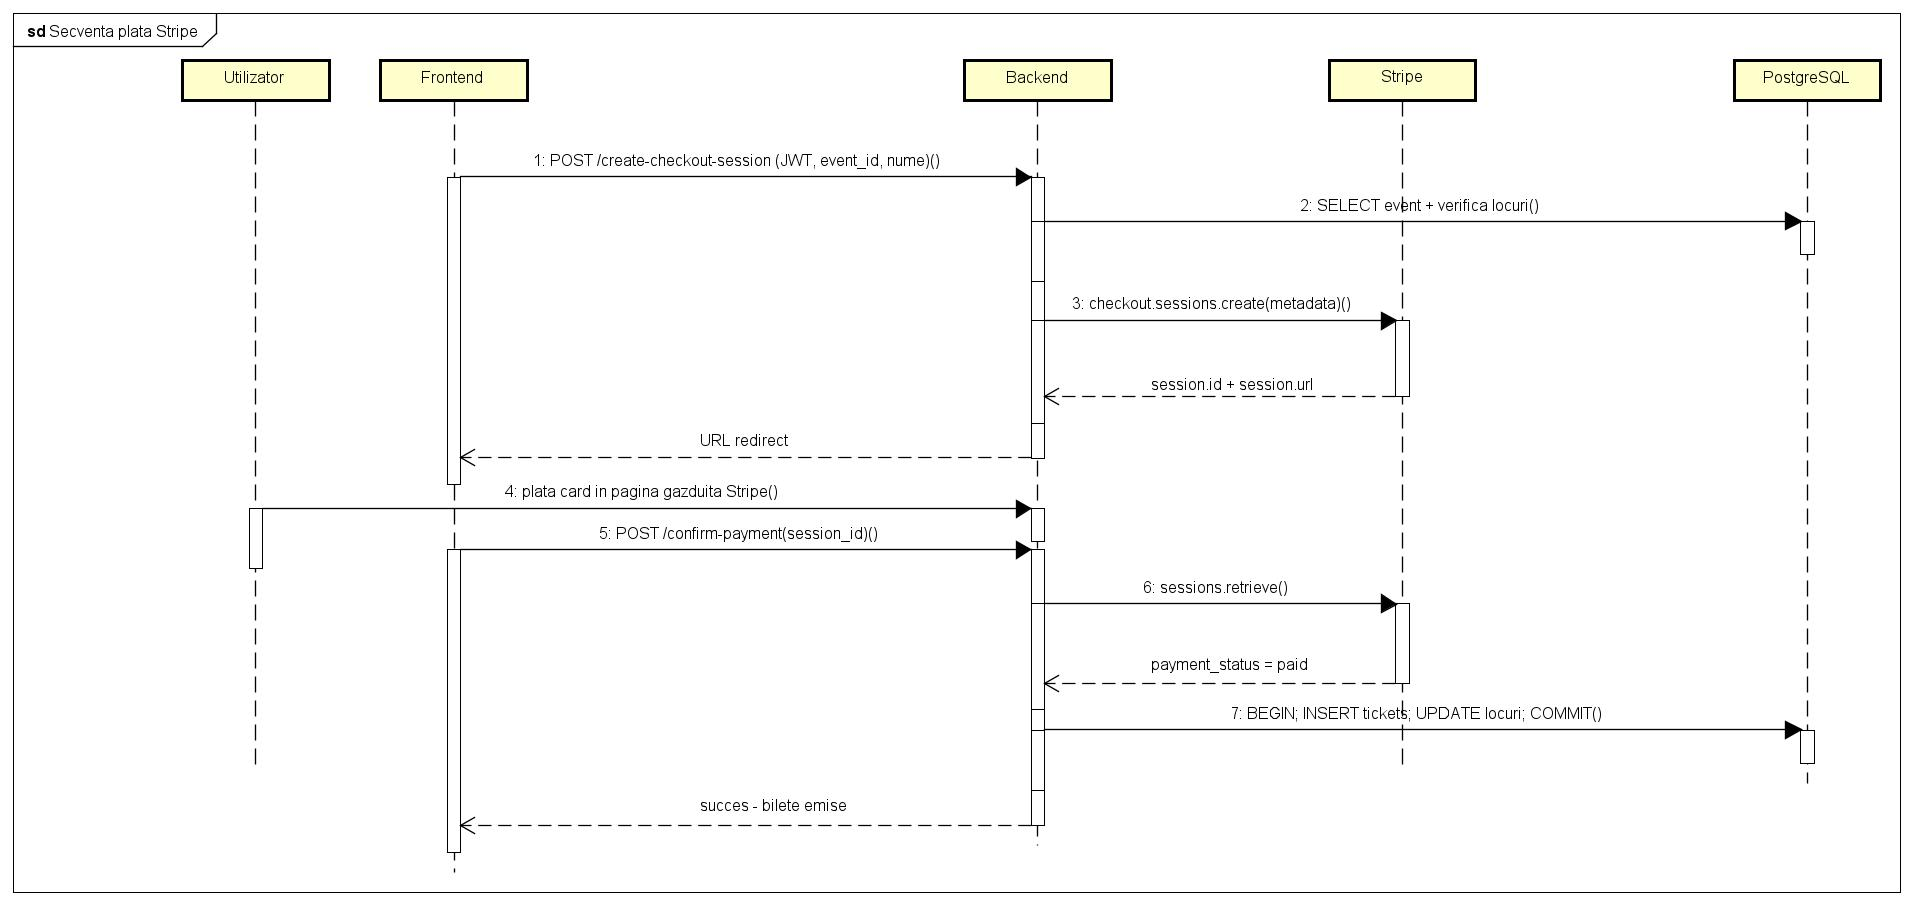
\includegraphics[width=1\textwidth]{Secventa plata Stripe.jpg}
	\caption{Diagrama de secventa - plata Stripe}
	\label{fig:l2f1}
\end{figure}


\subsection{Activitatea la check-in si admin}

Instructiuni inserare: Flowchart: admin selecteaza eveniment → lista participanti → validare bilet → UPDATE check\_in=true sau mesaj eroare

\begin{figure}[htbp]
	\centering
	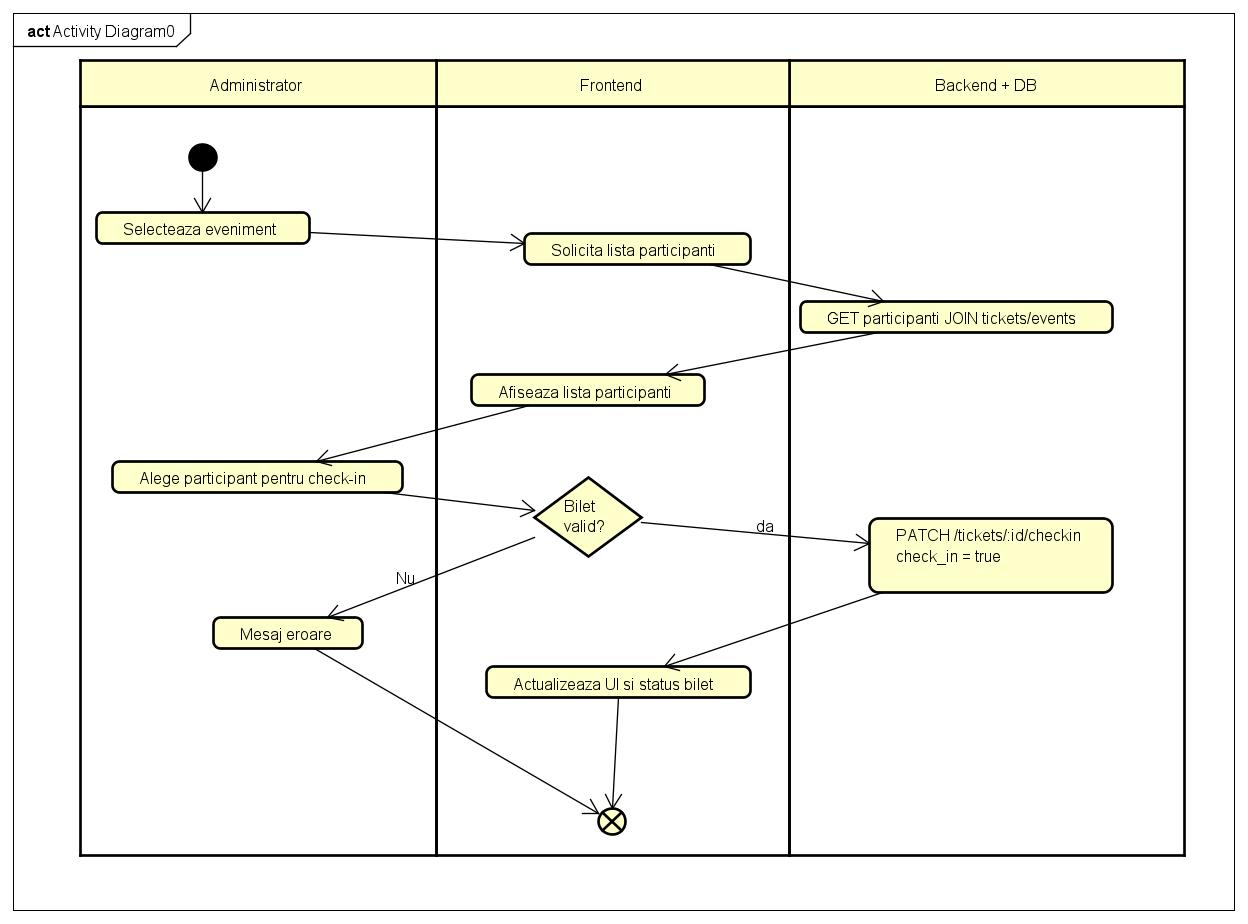
\includegraphics[width=1\textwidth]{Activity Diagram0.jpg}
	\caption{Diagrama de activitate - check-in}
	\label{fig:l2f1}
\end{figure}

\subsection{Proiectarea bazei de date}

Tabele principale: {\tt users, events, tickets, password reset tokens, registration verif}

Relatii: {\tt events} 1:N {\tt tickets; users} 1:N {\tt tickets} (ON DELETE SET NULL); {\tt users} 1:N token-uri reset; verificari ınregistrare temporare pana la confirmare. 

\begin{figure}[htbp]
	\centering
	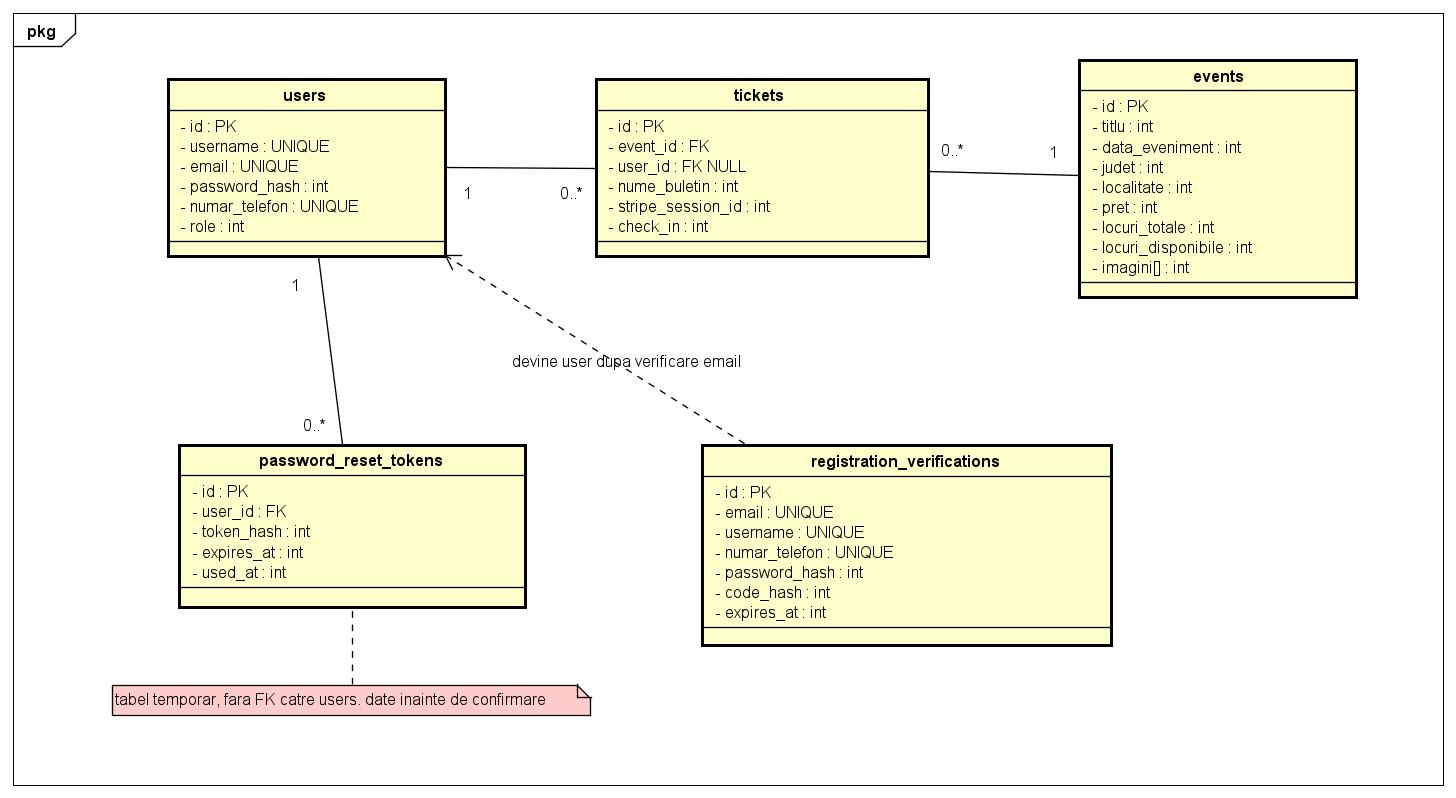
\includegraphics[width=1\textwidth]{Model de domeniu _ ERD ManFast.jpg}
	\caption{Diagrama entitate- relatie}
	\label{fig:l2f1}
\end{figure}


\section{Proiectarea bazei de date}





Tabele principale: {\tt user, events, tickets, password\_reset\_token, registration\_verifi}

Relatii: {\tt events} 1:N {\tt tickets; user} 1:N {\tt tickets} (ON DELETE SET NULL) {\tt user} 1:N token-uri reset si verificari inregistrare temporare pana la confirmare.




\section{Implementarea functionalitatilor cheie}
\subsection{Autentificarea si verificarea prin email}

Generarea codului si a hash-ului

\begin{lstlisting} 
	function genereazaCodVerificare() {
		return String(crypto.randomInt(100000, 1000000));
	}
	function hashCodVerificare(cod) {
		return crypto.createHash('sha256')
		.update(String(cod).trim()).digest('hex');
	}
\end{lstlisting}

La {\tt POST /register/verify}, codul este comparat cu {\tt code\_hash}, expirarea verificata, apoi utilizatorul inserat ın {\tt users}. Login-ul genereaza JWT: 

\begin{lstlisting}
	const token = jwt.sign(
	{ id: user.id, role: user.role },
	process.env.JWT_SECRET,
	{ expiresIn: '24h' }
	);
\end{lstlisting}

\subsection{Plati prin Scripe}

Crearea sesiunii Checkout (extras):

\begin{lstlisting}
	const session = await stripe.checkout.sessions.create({
		payment_method_types: ['card'],
		line_items: [{ 
			price_data: {
				currency: 'ron',
				product_data: { name: `Bilet - ${event.titlu}` },
				unit_amount: Math.round(Number(event.pret) * 100),
			}, 
			quantity: cantitate 
		}],
		mode: 'payment',
		success_url: `${frontendUrl}/payment-success?session_id={CHECKOUT_SESSION_ID}`,
		metadata: { 
			event_id, 
			user_id, 
			nume_participanti: JSON.stringify(nume)
		}
	});
\end{lstlisting}

{\tt confirm-payment} verifica˘ {\tt session.payment status} === ’{\tt paid}’, insereaza˘
cate un rand {\tt tickets} per nume si decrementeaza {\tt locuri\_disponibile} ıntr-o tranzactie.

\subsection{Gestionare evenimente}

Crearea evenimentului folosete Multer pentru imagini si validare judet¸ din lista fixa (42 judete). La INSERT, {\tt locuri\_disponibile = locuri totale}. Editarea permite adaugare incrementala de imagini. Stergerea elimina evenimentul si biletele asociate (CAS-CADE)

\subsection{Frontend}
	
{\tt AuthContext} stocheaza {\tt user} si {\tt token} ın {\tt localStorage}. {\tt apiFetch} atas¸eazaheader Authorization. Rute protejate: {\tt /profile, /my-tickets, /admin} (AdminRoute).



\section{Securitate}

\begin{itemize}
	\item Parole: bcrypt cost 10; niciodat\u a \^in clar \^in DB.
	\item JWT: secret separat de Stripe; expirare 24h.
	\item Coduri email \c si token reset: SHA-256 \^in DB.
	\item Rate limit: max 3 coduri / 15 min (produc\c tie); cooldown 60s retrimitere.
	\item CORS: doar \texttt{FRONTEND\_URL}.
	\item Admin: ultimul admin protejat la \c stergere/revocare.
	\item \c Stergere cont: confirmare parol\u a obligatorie.
\end{itemize}

Implementarea respecta recomandarile OWASP [3] pentru autentificare si gestionarea sesiunilor ın contextul unei aplicat¸ii web educationale/prototip production-ready.

\section{Scenarii de utilizare pe tipuri de evenimente}

Aceasta sectiune descrie modul ın care aceleasi functionalitati ale platformei sunt valorificate ın scenarii reprezentative. Scopul este de a demonstra flexibilitatea modelului simplu eveniment–bilet, fara a impune module separate per domeniu.

\subsection{Scenariul 1: Conferinta universitara}

Context: Facultatea organizeaza o conferint¸ a stiintifica cu 150 de locuri, taxa de participare 120 RON, desfasurare ın Constanta.

\hspace*{2ex} \textbf{Pași organizator:}
\begin{enumerate}
	\item Administratorul creează evenimentul: titlu, descriere (program, speakeri), dată, județ Constanța, localitate, locație (sală), preț 120, locuri 150, durată 8 ore, imagini (banner conferință).
	\item Publică link-ul către pagina principală; participanții filtrează după dată sau județ.
	\item Monitorizează {\tt locuri\_disponibile} și lista participanților.
	\item La intrare, efectuează check-in pe baza numelui de pe bilet.
\end{enumerate}

\textbf{Pași organizator:} Pasi participant: ınregistrare cont, verificare email, cumparare bilet nominal, prezentare la receptie. Biletul din “Biletele mele” confirma plata si identitatea.

\subsection{Scenariul 2 in care concertul este in aer liber}

\textbf{Context:} Asociatie culturala organizeaza un concert local, 500 locrui, bilet 50 RON, galerie foto artisti.

\textbf{Particularitati:} Galeria cu multiple imagini sporet¸e atractivitatea paginii de detalii. Filtrarea pe judet¸ ajuta publicul din zona. Vanzarea poate include mai multe bilete ıntr-o singura tranzactie Stripe (familie, grup de prieteni), fiecare nume completat corespunde unui bilet nominal.

\textbf{Limitari actuale:} Nu exista categorii de pret¸ (VIP, standard) sau harta locurilor — extensii posibile prin adaugarea unui camp {\tt tip\_bilet} ın schema bazei de date.

\subsection{Scenariul 3: Meeting corporate / training}

\textbf{Context:} Firma de IT organizeaza un workshop de o zi, 30 locuri, participare gratuita sau cu pret simbolic

Context: Club sportiv local, turneu cu taxa de ˘ ˆınscriere, necesitate nume conform buletinului.
{Utilizare:} Chiar si la pret¸ mic, Stripe permite monetizare. Alternativ, organizatorul poate
seta pret 1 RON pentru testare. Check-in-ul din admin ofera lista de prezenta pentru raport intern. Verificarea email la ınregistrare reduce ınscrierile fictive.

\subsection{Scenariul 4: Competitie sportiva amatoriala}

\textbf{Context:} Club sportiv local, turneu cu taxa de ınscriere, necesitate nume conform buletinului.

\textbf{Utilizare:} Campul {\tt nume} buletin la cumparare capteaza numele participantului. Check-in manual valideaza prezenta. Aceasta nisa folosete aceleasi mecanisme ca conferinta, fara tabele suplimentare pentru echipe sau clasamente. 

\subsection Matricea functionalitatilor si scenarii

\begin{table}[htbp]
	\centering
	\begin{tabular}{|l|c|c|c|c|}
		\hline
		\textbf{Funcționalitate} & \textbf{Conf.} & \textbf{Concert} & \textbf{Meeting} & \textbf{Sport} \\ \hline
		Filtrare județ/dată & Da & Da & Da & Da \\ \hline
		Galerie imagini & Da & Da & Opțional & Opțional \\ \hline
		Plată Stripe RON & Da & Da & Da & Da \\ \hline
		Bilete multiple / tranzacție & Da & Da & Rar & Da (echipe mici) \\ \hline
		Check-in admin & Da & Da & Da & Da \\ \hline
		Nume nominal (buletin) & Opțional & Opțional & Opțional & Da \\ \hline
	\end{tabular}
	\caption{Funcționalități utilizate în scenarii}
	\label{tab:functionalitati_scenarii}
\end{table}

\subsection{Modelul unificat de date}

Decizia de a nu specializa tabelele per tip de eveniment (conferint¸a vs. concert) simplifica mentenanta si permite unui singur panou admin sa gestioneze toate formatele. Campurile {\tt titlu, descriere, data eveniment, judet, pret, locuri totale si imagini} sunt suficient de generice; semantica (“taxa conferinta” vs. “bilet concert”) este pur textuala, definita de organizator.

Aceste scenarii pot fi reproducte ın cadrul demonstratiei aplicatiei si documentate prin capturi de ecran ın capitolul 4.

\section{Fragmente suplimentare de implementare}
\subsection{Rate limiting la inregistrare}

Functia depasesteLimitaCoduri limiteaza abuzul de retrimitere cod email ın productie:

\begin{lstlisting}
	function depasesteLimitaCoduri(row) {
		if (isDev) return null;
		
		const secundeDeLaUltimulCod =
		(Date.now() - new Date(row.last_code_sent_at).getTime()) / 1000;
		
		if (secundeDeLaUltimulCod < COOLDOWN_RETRIMITERE_SEC) {
			return { status: 429, error: 'Asteapta inainte de un cod nou.' };
		}
		
		if (inFereastraDe15Minute(row.last_code_sent_at)
		&& row.codes_sent >= MAX_CERERI_COD_15_MIN) {
			return { status: 429, error: 'Prea multe cereri de cod.' };
		}
		
		return null;
	}
\end{lstlisting}

ˆIn modul development ({\tt NODE ENV} diferit de ’{\tt production}’), limitarea este dezactivata pentru a facilita testarea repetata fluxului de ınregistrare fara a astepta cooldown-ul de 60 de secunde

\subsection{Middleware autentificare JWT}

Middleware-ul {\tt authenticateToken} extrage token-ul din header {\tt Authorization}: {\tt Bearer}, verifica semnatura cu JWT SECRET si ataseaza req.user pentru rutele protejate:

\begin{lstlisting}
	function authenticateToken(req, res, next) {
		const authHeader = req.headers['authorization'];
		const token = authHeader && authHeader.split(' ')[1];
		
		if (!token) return res.status(401).json({ error: 'Token lipsa' });
		
		jwt.verify(token, process.env.JWT_SECRET, (err, user) => {
			if (err) return res.status(403).json({ error: 'Token invalid' });
			req.user = user;
			next();
		});
	}
\end{lstlisting}

{\tt requireAdmin} verifica suplimentar {\tt req.user.role === ’admin’}, returnand 403 pentru utilizatori obisnui. Aceasta separare permite reutilizarea autentificarii pe rute mixte (ex. /auth/me vs. /events POST).

\subsection{Validare evenimente la creare}

La {\tt POST /events}, backend-ul valideaza judetul din lista fixa, pretul pozitiv, locuri disponibile si proceseaza upload-ul Multer:

\begin{lstlisting}
	const JUDETE_VALIDE = ['Alba', 'Arad', ..., 'Vaslui', 'Vrancea'];
	
	if (!JUDETE_VALIDE.includes(judet)) {
		return res.status(400).json({ error: 'Judet invalid' });
	}
	
	const locuriTotale = parseInt(locuri_totale, 10);
	
	if (isNaN(locuriTotale) || locuriTotale < 1) {
		return res.status(400).json({ error: 'Locuri invalide' });
	}
\end{lstlisting}

Imaginile sunt salvate ın {\tt uploads/events/} cu nume unic (timestamp + random), iar URL-urile relative sunt stocate ın coloana {\tt imagini} de tip {\tt TEXT[]}.

\subsection{Componenta AdminRoute (frontend)}
 Ruta {\tt /admin} este protejata pe client prin verificarea rouluiu din contex:
 
 \begin{lstlisting}
 	function AdminRoute({ children }) {
 		const { user, loading } = useAuth();
 		
 		if (loading) return <CircularProgress />;
 		
 		if (!user || user.role !== 'admin') {
 			return <Navigate to="/login" replace />;
 		}
 		
 		return children;
 	}
 \end{lstlisting}
 
 Protect¸ia pe client este complementara, nu substitut pentru requireAdmin pe server — orice apel API admin fara token valid este respins indiferent de manipularea rutei React. 
 
 \subsection{Gestionare erori si feedback utilizator}
 
 Frontend-ul centralizeaza apelurile API ın {\tt apiFetch}, interpretand raspunsurile JSON si afiseaza mesaje Material UI ({\tt Alert, Snackbar}). Codurile HTTP 400/401/403/429/500 sunt mapate la texte ın romana ın componentele de formular.
 
 Backend-ul returneaza structuri consistente {{\tt error: string} } evitand expunerea stack trace ın productie. Logging-ul pe consola ( {\tt console.error}) assista debugging-ul ın development.

 Aceste fragmente ilustreaza detalii de implementare care completeaz a diagramele si tabelele API, oferind cititorului o imagine concreta a codului sursa ManFast. 
 
 \section{Modelul relational - detaliu tavele}
 \subsection{Tabel user}
 
 Stocheaza conturile utilizatorilor. Campuri: {\tt id} (SERIAL PK), {\tt username} (UNIQUE), {\tt email} (UNIQUE), {\tt password\_hash, numar\_telefon} (UNIQUE), {\tt role} ({\tt user—admin}), {\tt created\_at}. Rolul determina accesul la  {\tt /admin}.
 
 Evenimentele publicate de administratori: {\tt titlu, descriere, data eveniment, judet,
 localitate, locatie} (string compus pentru afis¸are), {\tt pret, locuri totale, locuri disponib imagini} (TEXT[]), {\tt durata ore}. La creare,{\tt locuri disponibile = locuri totale}. Filtrarea pe home exclude evenimente expirate ({\tt data + durata < NOW()}).
 
\subsection{Tabele auxiliare}
	 
{\tt registration\_verifications} — stocare temporara ınregistrarilor pana la cod email. 
{\tt password\_reset\_tokens} — token hash SHA-256, expirare 1h, used at la consum.
	
\section{API REST - referinta}

Prefix: {\tt /api}. Tabelul 3.3 listeaza endpoint-urile de autentificare.

\begin{table}[htbp]
	\centering
	\begin{tabular}{|>{\ttfamily}p{5.5cm}|c|l|}
		\hline
		\textbf{Endpoint} & \textbf{Metodă} & \textbf{Descriere} \\ \hline
		/auth/register & POST & Trimite cod verificare email \\ \hline
		/auth/register/verify & POST & Confirmă cod, creează cont \\ \hline
		/auth/register/resend & POST & Retrimite cod \\ \hline
		/auth/login & POST & Autentificare, returnează JWT \\ \hline
		/auth/me & GET & Utilizator curent (JWT) \\ \hline
		/auth/profile & PUT & Actualizare profil \\ \hline
		/auth/password & PUT & Schimbare parolă \\ \hline
		/auth/account & DELETE & Ștergere cont (parolă) \\ \hline
		/auth/forgot-password & POST & Solicitare reset \\ \hline
		/auth/reset-password & POST & Parolă nouă cu token \\ \hline
		/auth/admin/create & POST & Promovare admin \\ \hline
		/auth/admin/revoke & POST & Revocare admin \\ \hline
	\end{tabular}
	\caption{Endpoint-uri autentificare}
	\label{tab:endpoints_auth}
\end{table}

\begin{table}[htbp]
	\centering
	\begin{tabular}{|>{\ttfamily}p{8cm}|c|l|}
		\hline
		\textbf{Endpoint} & \textbf{Metodă} & \textbf{Descriere} \\ \hline
		/events & GET & Listă publică evenimente viitoare \\ \hline
		/events/:id & GET & Detalii eveniment \\ \hline
		/events & POST & Creare (admin) \\ \hline
		/events/:id & PUT & Editare (admin) \\ \hline
		/events/:id & DELETE & Ștergere (admin) \\ \hline
		/events/admin/list & GET & Listă admin \\ \hline
		/tickets/create-checkout-session & POST & Sesiune Stripe \\ \hline
		/tickets/confirm-payment & POST & Confirmare plată \\ \hline
		/tickets/my-tickets & GET & Biletele utilizatorului \\ \hline
		/tickets/admin/participants & GET & Participanți (admin) \\ \hline
	\end{tabular}
	\caption{Endpoint-uri evenimente și bilete}
	\label{tab:endpoints_evenimente_bilete}
\end{table}

\section{Configurare si deployment}
\subsection{Variabile de mdiu backend}

{\tt DB *, JWT SECRET, STRIPE SECRET KEY, FRONTEND URL, SMTP *, MAIL FROM,
ADMIN AUTHORIZATION PASSWORD}. Frontend: {\tt VITE API URL}.

\subsection{Migrari baza de date}

Scripturi npm: {\tt setup-db, migrate-judet-localitate, migrate-password-reset, migrate-email-verification, migrate-multi-tickets.} Schema completa ın {\tt database/schema.sql.}

\subsection{Flux instalare}

\begin{enumerate}
	\item \textbf{PostgreSQL:} \texttt{CREATE DATABASE manfast}
	\item \texttt{cd backend \&\& npm install \&\& npm run setup-db}
	\item Rulare migrări incrementale dacă proiect existent
	\item \texttt{npm run dev} backend; \texttt{cd frontend \&\& npm run dev}
	\item \textbf{Promovare admin:} \texttt{npm run promote-admin -- email@exemplu.com}
\end{enumerate}

\subsection{Componente frontend}

\subsubsection{Rute React Router}
\texttt{/}, \texttt{/login}, \texttt{/register}, \texttt{/forgot-password}, \texttt{/reset-password}, \texttt{/events/:id}, \texttt{/profile}, \texttt{/my-tickets}, \texttt{/payment-success}, \texttt{/admin} (\texttt{AdminRoute}).

\subsubsection{Context autentificare}
\texttt{AuthContext} expune \texttt{user}, \texttt{token}, \texttt{login}, \texttt{logout}, \texttt{updateUser}. \textbf{Token JWT în localStorage}. La \texttt{apiFetch}, header \texttt{Authorization: Bearer}.

\subsubsection{Temă vizuală}
\texttt{darkTheme.js} — paletă cyan pe fundal întunecat. Componente refolosibile: \texttt{AuthCard}, \texttt{PageContainer}, \texttt{EventListItem}, \texttt{StatusChip}.


\subsection{Confirmare plată — pseudocod}

\begin{lstlisting}[mathescape=true]
	BEGIN transaction
	existing = SELECT tickets WHERE stripe_session_id
	IF existing.count >= cantitate THEN COMMIT; RETURN dejaProcesat
	FOR nume IN numeDeInserat:
	INSERT INTO tickets (event_id, user_id, nume_buletin, ...)
	UPDATE events SET locuri_disponibile -= count
	COMMIT
\end{lstlisting}

\noindent Idemponteuța: reapelarea \texttt{confirm-payment} cu același \texttt{session\_id} nu dublează biletele.


\subsection{Testare manuală}

Scenariu recomandat pentru demonstrație:
\begin{enumerate}
	\item înregistrare + cod email;
	\item login;
	\item filtrare evenimente;
	\item cumpărare bilet Stripe test \texttt{4242...};
	\item verificare ,,Biletele mele``;
	\item promovare admin;
	\item publicare eveniment;
	\item check-in;
	\item editare profil;
	\item ștergere cont test.
\end{enumerate}

Aceste detalii completeaza documentatia tehnica necesara pentru ıntelegerea si reproductibilitatea solutiei ManFast.